\documentclass[doc,12pt,floatsintext]{apa7}
%\usepackage{setspace}
%\singlespacing
\usepackage{subfigure}
%\usepackage{ctable}
\usepackage{array}
\usepackage[american]{babel}
\usepackage{csquotes} 
\usepackage[backend=biber, style=apa]{biblatex}
\DeclareLanguageMapping{american}{american-apa} 
\addbibresource{bibfile.bib} 
\usepackage[T1]{fontenc} 
\usepackage{mathptmx} 
\title{Computational representation of social complexity for decision making: the case of climate change, migration, and social conflict}

\shorttitle{Computational representation of social complexity} % The short title for the header
\author{Jose Manuel Magallanes}
% \duedate{April 20, 2024}
% \date{January 17, 2024} The student version doesn't use the \date command, for whatever reason
\authorsaffiliations{Instituto de Analítica Social e Inteligencia Estratégica (PULSO PUCP), Pontificia Universidad Católica del Perú - PUCP}

\authornote{\scriptsize
   \addORCIDlink{José Manuel Magallanes}{0000-0002-2593-0859}
   
Correspondence concerning this article should be addressed to José Manuel Magallanes, PhD., Professor at Departmento de Ciencias Sociales, and Director of PULSO-PUCP, Pontificia Universidad Católica del Perú, Av. Universitaria 1801, San Miguel - Lima, Perú.  E-mail: \texttt{jmagallanes@pucp.edu.pe}}
  

\abstract{This chapter illustates how computer simulations can help us foresee critical situations  in populations where climate change may cause water scarcity. In particular, we exemplify a city in the central Andes of Peru whose conditions related to deglatiation, urbanization, and population growth, may bring water scarcity. The main technique used is agent-based modeling, which will combine quantitative and qualitative information. The results show possible scenarios of water scarcity leading to drastic migration and social conflict, a situation not yet evident as a public problem. This work provides  recommendations for this likely and undesired scenario.}

\keywords{Social complexity, agent-based modeling} % If you need to have keywords for your paper, delete the % at the start of this line

\usepackage{Sweave}
\begin{document}

\Sconcordance{concordance:ComplexityComputationalMagallanes.tex:ComplexityComputationalMagallanes.Rnw:1 %
31 1 1 0 551 1}

\maketitle % This tells LaTeX to make the title page

\section{Introduction} 

Social problems are mainly complex. That is, combine environmental, technological, psychological, social, political, and cultural issues. This complicates policy  and political decision making as one branch alone of the government can not solve public problems effectively, but involving several branches and multilevel decision makers will not make the discussion more efficient. 

This chapter presents social simulations via agent-based modeling (ABM). As \textcite{macy_factors_2002} propose, ABMs will allow the social scientists to change their  modeling efforts to represent societies as interactions among variables into a different paradigm where social life can finally be represented as interactions among adaptive agents who influence one another in response to the influence they receive.

This chapter exemplifies the use of ABMS to understand the interaction of climate change and population growth in a small-sized city. The ABM will allow us to envision possible futures as climate change trends affect water availability, the growth of the population urbanizes neighboring rural areas, and people need to decide in the future whether to stay or leave. 

Water scarcity and droughts have an slow onset \parencite{singh_losses_2021}, so as time passes by, the majority of urban and rural settlers do not pay much attention to this issue. However, if we look into the future the absence of water may affect the decision of settlers in the urban and rural areas in different ways that need a preliminary answer:

\begin{itemize}
\item Is it possible that drastic migration patterns appear as people do not find water?
\item Is it possible the emergence of social conflict in the area among the people that can not migrate and find themselves in a place with no water?
\end{itemize}

The purpose of an ABM is to serve as an input for  anticipatory and participatory political decisions \parencite{daquino_role_2002}. The presence of different actors with different goals and beliefs under stress due to the environmental conditions makes it challenging for mainstream modeling techniques based on variables are limited to provide the right guidance, so this work hopes to contribute methodologically in the coming discussion of the future of this city. There are certainly many computational modeling approaches---e.g. system dynamics or discrete systems simulations---that deal with organizational complexity. However, key concepts such as learning and emergence can only be modeled, arguably, through the use of ABMs \parencite{cioffi-revilla_introduction_2014,miller_complex_2007,gilbert_simulation_2005,epstein_growing_1996}. As with all modeling techniques, ABMs need to capture the most basic variables and processes that could explain a particular phenomenon, while making all building assumptions explicit and transparent, and producing outcomes valid and of interest to the scientific and policy community. In contrast to other techniques, ABMs are virtual laboratories that allow their components to have different behaviors, reactions, and to be aware of only limited information. In particular, ABMs are useful in the social sciences when a particular social theory can be enacted through coding. You all can then see how the model behaves as the building parameters of the theory are manipulated \parencite{miller_complex_2007,epstein_growing_1996}. Besides, ABM allows for the inclusion of complementary theories and models to carefully enrich the original theory, allowing the creation of different scenarios.

   

Climate change is a major social concern that needs profound reflection for the future of humanity; particularly if it affects the availability of water \parencite{robinson_water_2023}. But even if climate change were not a concern,  population and city growth by themselves will challenge the best efforts in water management \parencite{alfarra_nbs_2018}. 

% , whihas been under study by different scholars and institutions whose objectives are similar yet lacking inter disciplinary integration. Different public  research institutes are working to produce either glaciological, hydrological or climatological updates on the area; isolated researchers are doing small-scale models to whether alert of different local water risks or propose adaptation programs in the communities more likely to be affected by the nature trends.

The application presented is based on the area that depend on the water from the Shullcas River in the central Andes of Peru. The Shullcas river is a proglacial river originated from the meltings of the Huaytallana tropical glacier, a the kind of glacier more likely to disappear if global warming trends are unaltered \parencite{willige_explainer_2023}. The area includes rural and urban settlers that make exclusive use of the water from that river. The area has a positive population growth, with a marked tendency to urbanize the rural area located on the Huaytapallana's foot and skirt. Given this context, this example serves the current studies on computational representation of social complexity: 

\begin{itemize}
\item First, the object of study is not one particular kind of population (as it is the case in most studies) but it studies simultaneously vulnerable but not marginal rural populations, and an urban population of the close metropolitan area; so the water issues will be of concern to two different kind of groups with different necessities on water, which may be the starting point for inter group conflict \parencite{bar-tal_intergroup_2011}. 
\item Second, this ABM will include the effect of a glacier in the water supply for the social system, facilitating the analysis of similar systems by separating the precipitation (rainfall and snow melt). 
\item Third, the watershed under analysis may be a representative case for the whole Andes chain, as it is at the center, among the dry biggest cities on the west and the sparsely inhabited Amazon jungle to the east. 
\item Fourth, it integrates and harmonize current modeling efforts on the glacier melting trend, the hydrology dynamics and the social behavior; making our work more challenging as these systems have never been integrated before bringing into question the validity of our results. 
\item Finally, and related to the previous point, the issue is not of particular concern neither to the majority of the population nor to the political authorities; it looks as though nobody wants to touch the situation as it may collide with the current way people live and benefit. This work also continued with the best practices in computational social science (CSS) research used by the previous studies, as it  integrated the complex adaptive systems approach \parencite{miller_complex_2007}, the CSS consolidated techniques \parencite{cioffi-revilla_introduction_2014}, and ethnographic work \parencite{crate_anthropology_2009}.
\end{itemize}

\section{Literature Review}

Research interests dealing with modeling climate change are varied, but they tend to have a common interest in rural populations, especially vulnerable and located in developing countries. \Textcite{ziervogel_agent-based_2005}  focuses on modeling decision-making and forecasting of farmers in Lesotho, in an scenario where official forecasts, besides poorly done, are not diligently nor appropriately disseminated towards these end-users, making them more vulnerable as loses due to poor information endanger the farmers' survival. A similar research is found in Bharwani et al. \parencite{bharwani_multi-agent_2005} for smallholder farmers in a village in Vhembe district, Limpopo Province, South Africa. 

Modeling using ABMs more comprehensive approaches are found in Kniveton et al. \parencite{kniveton_agent-based_2011} and Hailegiorgis \parencite{hailegiorgis_computational_2013}. The former has Burkina Fasso as its case study, investigating the role of the environment in the decision to migrate using scenarios of future demographic, economic, social, political, and climate change in a dry land context. In that work, it is found that change to a drier environment produces the largest total and international migration fluxes when combined with changes to inclusive and connected social and political governance, while the lowest international migration flows are produced under a wetter climate with exclusive and diverse governance scenarios. And the latter focuses on the South Omo zone in southern Ethiopia, modeling how the current surge in large-scale land acquisition might affect rural livelihood. In this work,  Hailegiorgis found that (i) the occurrence of drought affects their adaptive capacity and forces migration; (ii) increasing the magnitude of expansion of large-scale land acquisition aggravate dispossession and increase migration of rural households; and (iii) capacity building and relief support in the time of extreme events minimizes migration. 

% The ABMs used diverse platforms; for  (Netlogo \parencite{wilensky_introduction_2015}, Mason \parencite{luke_mason_2015}, and AnyLogic \parencite{anylogic_2015}).
% \par
As it is clear so far, climate change stresses the place where human activities are carried out, thus deteriorating the quality of the environment of these populations forcing them to make different decisions, which, as Hirschmann proposes \parencite{hirschman_exit_1970}, can be categorized as {\emph exit}, {\emph voice} and {\emph loyalty}. The previous cases speak of exit, as people emigrate looking for better conditions as the climate threatens their well-being; but, the confrontational and loyalty dimensions in social complexity issues also need to be analyzed under climate change effects. However, loyalty and voice seem to be less treated from the global computational social science community, which should be considered quite shocking as reports related to climate change and conflicts are abundant \parencite{hendrix_climate_2012,hsiang_quantifying_2013,steinbruner_climate_2013}. Related to conflict and climate change, Piontek \parencite{piontek_impact_2010} studies the Nile River, which serves 10 countries in Africa, seeking to understand, via computational modeling, how the interaction between humans and the environment may lead to conflict or cooperation. In this work, the author found that climate change can alter conditions for conflict and cooperation, but it might not the immediate cause for those issues. Nevertheless, the most outstanding work related to climate change and the emergence of conflicts can be found in the works produced at the Center for Social Complexity at George Mason University' projects funded by the Multidisciplinary University Research Initiative (MURI) and Cyber-Enabled Discovery and Innovation (CDI) programs \parencite{cioffi-revilla2010,hailegiorgis_agent_2010,kennedy_agent-based_2010}. They focuse on the complex interaction of pastoral groups with their environment and other emerging external actors in east Africa finding that increased seasonal rainfall variability and droughts create tremendous stress on pastoral groups and challenges their long-term resilience and adaptive response mechanisms, thus concluding the population's relation to the carrying capacity seems to be the major factor affecting cooperation and conflict
% 




\section{Methodology}

% This work has the general goal of producing a base case interdisciplinary model to represent \emph{a possible} future for Huancayo as the water balance becomes insufficient to satisfy the population's needs. We consider this model as a coupled human-natural system, where the model keeps the current trends in both systems and sees whether it is possible to see emigration and social conflict emerge.
% 
% The product of this work is an agent-based model programmed in Netlogo \parencite{wilensky_introduction_2015}, which will follow a complex adaptive systems approach, when needed. The model respects particular characteristics of complex adaptive systems: there are many agents interacting dynamically, the agents have bounded rationality, i.e., only aware of local information, the agents have ways to establish networks which helps them get information, and history matters as path dependence emerges from the agent decisions. However, this complexity is well \emph{encapsulated} into the model, so the non-expert user can interact with it and even contribute to its improvement. 

This ABMS is very abstract.  It is built to capture the  relationships that answer our questions and be useful for policy discussion. Thus, we have two sytems, the social and the natural one. The systems interact and the ABM will see if  migration and conflict become more likely as time goes by. This is represented in Figure \ref{scheme}.

\begin{figure}[ht]
  \centering
  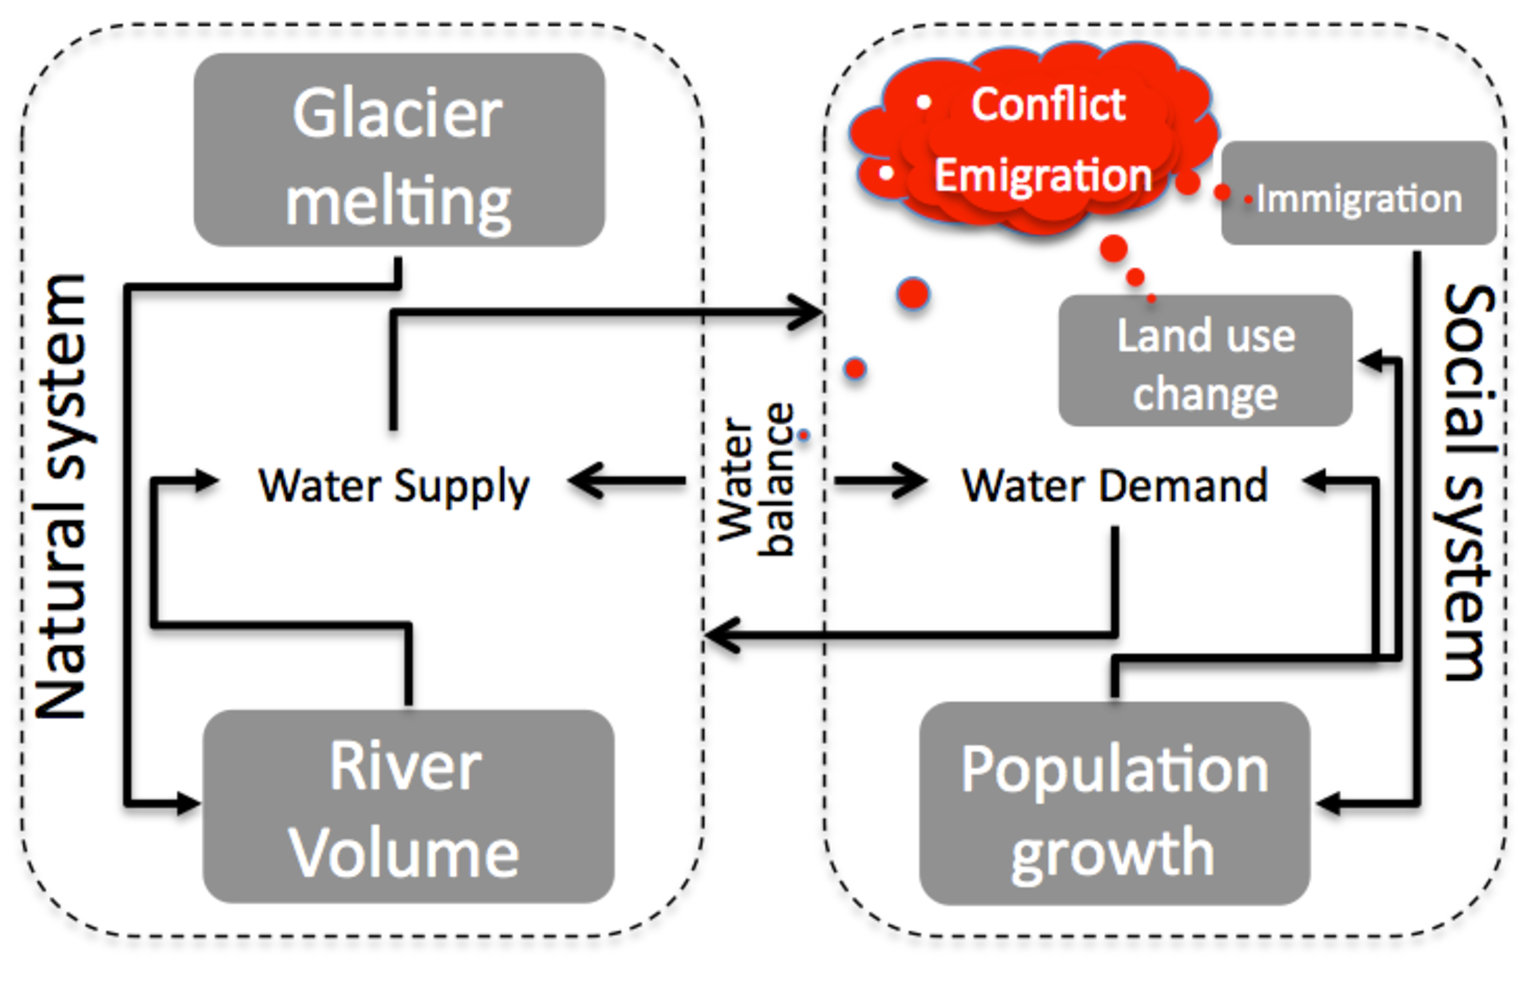
\includegraphics[width=0.7\textwidth]{modelsummaryGraph}
  \caption[Basic model abstraction]{Basic model abstraction. The red elements represent the potential outcomes if the other elements keep the current trends}
  \label{scheme}
\end{figure}


As it can be seen in Figure \ref{scheme}, the natural system focuses on the water supply, as it is the key trigger factor for the social issues of interest in this chapter.  The current studies of the area propose both a decreasing supply of rainfall, and forecast the complete retreat of the glacier, which will affect the balance negatively \parencite{carlos_riesgos_2012,lopez-moreno_recent_2014}. One obstacle for a more precise model is the lack of information on the snow melt supply; however, this value was bounded based  on  expert opinions\footnote{I thank Bryan Mark from Ohio State University for his input on this.}.
% 
On the other hand, water demand comes from the social system, which is represented by two subsystems, rural and urban. The basic process in both sub systems is population growth\footnote{The population growth parameter was simply computed from the census data available since 1981 at the Peruvian National Institute of Statistics (INEI) website.}, that is, eventually there will be not enough water supply for the population's demand. We explore emigration as a particular response (other responses have not been considered at all): there are not many Andean cities having positive population growth but the area under study is one of them, so making a case for the opposite phenomenon is politically important. Other demographic information is fed into the model (working, educational and marital status).


% Following the field work on this area, this model tries to give the agent options to avoid migration as water scarcity increases, but the limited local space and agent\textquotesingle s satisfaction will eventually leave him no more option than migrate. Another set of demographic variables for the agents are their working, educational and marital status, which are used in the moment the urban agent decide \emph{where} to migrate, that is, those values constrain their free will to chose between moving to the coast or the jungle. We have also considered the immigration parameters in this area, considering that currently Huancayo hosts immigrants from poorer communities nearby, which will be a key factor for conflict to emerge. Precisely speaking, we present a basic heuristic to represent a situation when rural agents are eager to go into conflict due to the present of \emph{strangers} in their neighborhood during extreme water scarcity. As it is clear, conflict is a process that can emerge from the urban and rural area, while migration emerges from the urban area, and not from the rural area, following the results of our field work. However, for a rural agent to migrate, it first needs to have moved to the urban area; and for an urban agent to be perceived as a stranger by a rural one, it needs to have immigrated from another place and established its home in the neighborhood of a rural settler suffering water stress.
% 
\subsection{Hypothesis Operationalization}

As this work proposes that the research questions have affirmative answers, we propose the following operationalization of variables in the hypothesis, as described in Figure \ref{operational}:

\begin{figure}[h]
%%%\figSpace
  \centering
  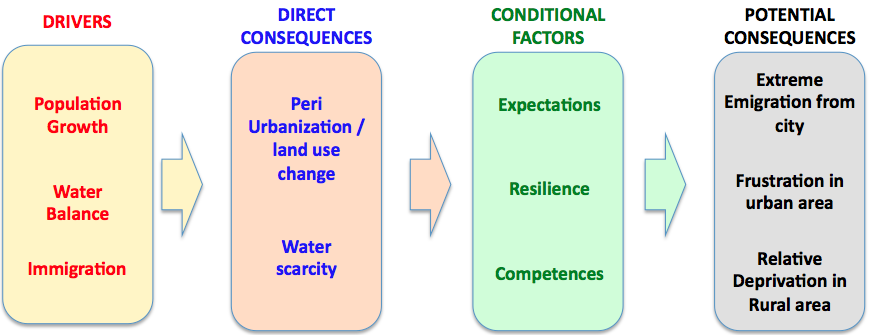
\includegraphics[width=0.9\textwidth]{operational}
  \caption[Operational Variables in Hypothesis]{Operational Variables in Hypothesis}
  \label{operational}
  %%%\figSpace % This adds separation
\end{figure}

The variables present a simple yet comprehensive process to study the potential for conflict and migration:
\begin{itemize}
\item The {\bf potential outcomes} are chosen as the representation of our framework \emph{exit, voice and loyalty}\parencite{hirschman_exit_1970}. In this case, \emph{exit} is represented by {\bf drastic migration}; \emph{loyalty} by the permanence in the ara (not shown); and \emph{voice} by expected reaction from the {\bf frustration} felt by urban people, or the {\bf relative deprivation} felt by rural people .

\item The {\bf drivers} clearly represent the current trends in the area, bith  in the social and natural dimensions. These trends are not altered in the ABM. The assumption that the trends can be extended into the future are based on the historical population growth and immigration. The water balance trend represents the other important driver, which will be represented by water supply and demand. Water supply will be based on the contribution of the glacier Huaytapallana.

\item The {\bf direct consequences} are the clear results of the unaltered trends.The ABM includes the two most clear direct consequences supported by the literature and field work \parencite{haller_huancayo_2013,Ho2012,haller_vivid_2012}. Water scarcity is a first expected outcome as the water balance and population growth trends remain unaltered. Water scarcity will become a major problem (as explained in \parencite{carlos_riesgos_2012} and detailed in the next chapter) in the near future, which will combine with population growth and, particularly, immigration to exacerbate peri urbanization and land use change \parencite{haller_huancayo_2013,haller_vivid_2012,Ho2012}.

\item The {\bf conditional factors} are processes that work at the individual level, and are the main sources of heterogeneity in the model. Every individual will need to find an particular response based on these factors. The factors have been selected from the classical work of Maslow \parencite{maslow_motivation_1987},  and its application in agent based modeling to understand conflictive situations \parencite{watkins_understanding_2008}. According to this individual level factors, we implemented a Bayesian mechanism to compute expectations, we carried out field work to uncover the local resilience, and made use of the census data to derive the competences of each individual. The competences reflect closely what determines the potential outcomes \parencite{watkins_understanding_2008}, that is, of water (physiological needs), work (safety needs), family (belonging needs) and education (for esteem and self-realization needs).

  % \begin{figure}[h]
  % %%%\figSpace
  %   \centering
  %   \includegraphics[width=0.65\textwidth]{maslow}
  %   \caption[Hierarchy of Maslow]{Pyramid showing Maslow's hierarchy of needs.}
  %   Source: From \url{http://psychclassics.yorku.ca/Maslow/motivation.htm}
  %   \label{maslow}
  %   %%%\figSpace % This adds separation
  % \end{figure}

\end{itemize}



\subsection{Field work}

We decided to organize an ad-hoc collection of information in situ as the ABM required some information for the agents not available neither on the literature nor the data. We needed to have a clearer idea on how the agents will react as water will become scarce in the rural and urban area. For that reason, we organized two research expeditions: One on the urban area and another in the rural area; Figure \ref{etno} show the area of study and the area cover for each expedition.

\begin{figure}[h]
%%%\figSpace
  \centering
  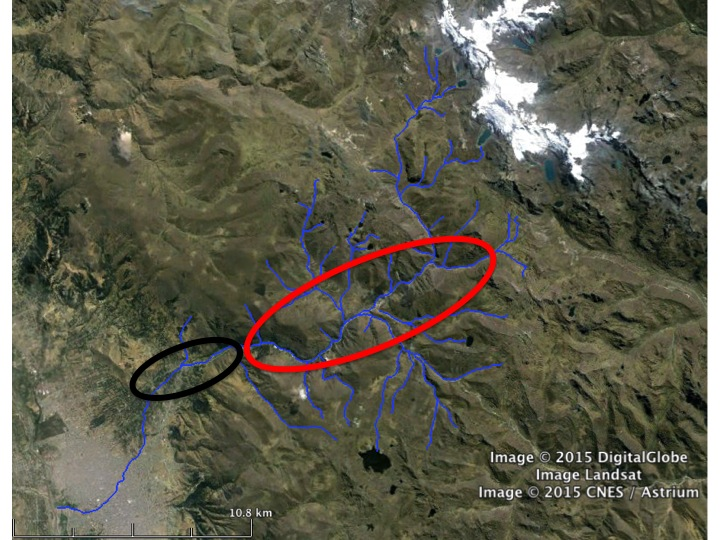
\includegraphics[width=0.75\linewidth]{etno}
  \caption[Map of Field work]{Map of Field work. The black oval is the area covered by the urban expedition and the red oval the area covered by the rural expedition}
  \label{etno}
  %%%%\figSpace % This adds separation
\end{figure}

The rural area has  the longest extension of land, but is also the less populated. The team made unstructured interviews with the goal of this expedition was to find out about: (i) the awareness of the water scarcity in the future; (ii) their need to migrate in case water scarcity reached unbearable leves; (iii) the possibility of taking some political action. The main findings were (i) person after person affirmed that drastic migration is not an option for the rural; (ii) the increasing presence of immigrants urbanizing the rural area represented an unappealing fact. The study also confirmed people were very aware of the progressive lack of water, but they believe this issue will be of more concern in the urban area. A couple of additional important facts were unveiled. First, they are sure that the urban needs of water will collide with the rural needs. They are not sure how much water will the growing city may need in the future. They are not confident local authorities will consider their opinion if the city needs more water. Second, they believe this generation of rural people will do their best effort to make a living in the rural area; but they are not very sure what would be the reaction of the future generations. They consider that the jungle represent an attractive destination for young unemployed people, but are afraid the attraction comes from easy-money and illegal activities.

The periurban expedition visited 65 families living in limit between the city and the rural area. A survey was designed and applied. The team designed a polietapic sampling design to include a representative sample of households of migranst and non-migrants in the urban settlements located along the peri urban area. The goal of this expedition was the same to the previous one. The information collected in the periurban area informed: (i) urban people have migration among their alternatives in case of lack of water; (ii) the urban settlers will look for a place nearby  to move in (they may need to get land closer to the rural area). It is worth noticing that all who said they would never migrate are immigrants; (iii) all  believe that they will feel frustrated if they have to stay in place with water scarcity. This expeditiom found that people in the periurban area did not start living in that zone but renting a place downtown, which was expensive, smaller and overcrowded, and, progressively, they moved (renting or buying) into the peri urban area as it represented a cheaper place to live. The strategy they followed to find a better place was a system of references, where family and friends were sharing their experience living outside the city center, even with lack of public utilities in the beginning. In case of searching for water, they say they will follow the same strategy (referencing system from relatives).

% The field work allowed me to complement the quantitative data available with some basic decision making mechanisms the rural and urban agents will adopt in case of this potential scenario. Besides, the information from the field work will help me introduce heterogeneity in the agents. We consider that within the limitations for this research we have enough information to produce an informative model that will bring sufficient information for policy makers to start anticipatory thinking in the problem this model presents.

\subsection{Modeling building}

The ABM simulates 50 years. Every time a complete cycle of the simulation is run, the history  advances six months.  So, this model will only run for 100 cycles. As each cycle represents six months, a cycle represents a season, which is either the \emph{dry season} (that goes from May to September) or the \emph{rainy season} (that goes from October to April). Figure \ref{flow1} reflects the flow of the code each cycle or season, a figure that also represents the translation of the concepts represented in the scheme \ref{scheme} on page \pageref{scheme} into computer logic.

\begin{figure}[ht]
%%\figSpace
\centering
  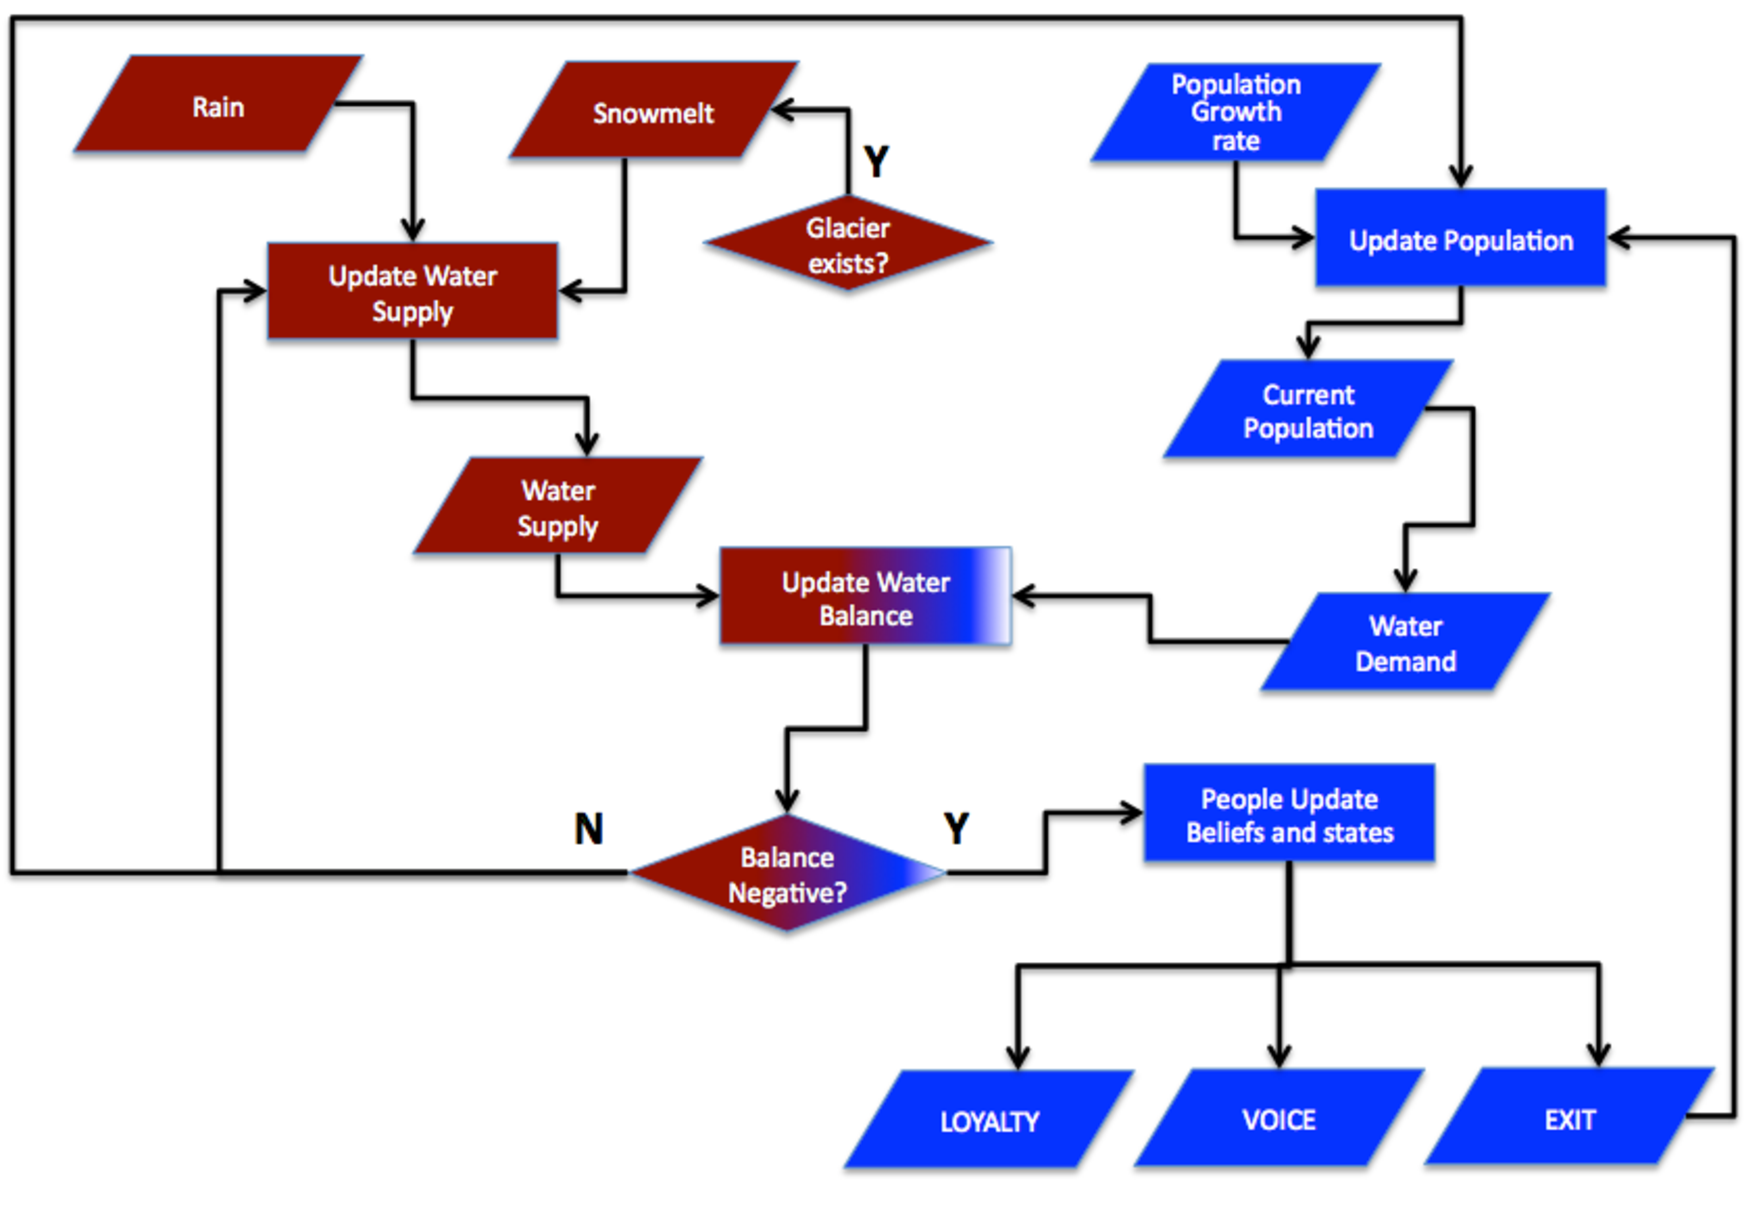
\includegraphics[width=0.8\textwidth]{flow1}
  \caption[Process Overview]{Process Overview. Color differentiates type of system (blue for  \emph{Social} and red for \emph{Natural}. A pass through this chart represents a six month \emph{season}.}
  \label{flow1}
  %%\figSpace
\end{figure}

Figure \ref{ruralLogic} is a flowchart representing the decision making of a rural agent. As it is shown in that figure, the decision flow starts when the agent detects scarcity. That detection is a particular computation following a Bayesian approach, which was the assumed as the mechanism to update beliefs. Once the agent detects scarcity, he will look for a place to move. As long as the agent detects scarcity where the agent is staying, the agent will move. The moving will end when the agent reaches the resilience limit. If the rural agent can migrate, the rural agent will migrate to the urban area. Agents that could not migrate are candidates to feel relatively deprived.

\begin{figure}[ht]
%%\figSpace
\centering
  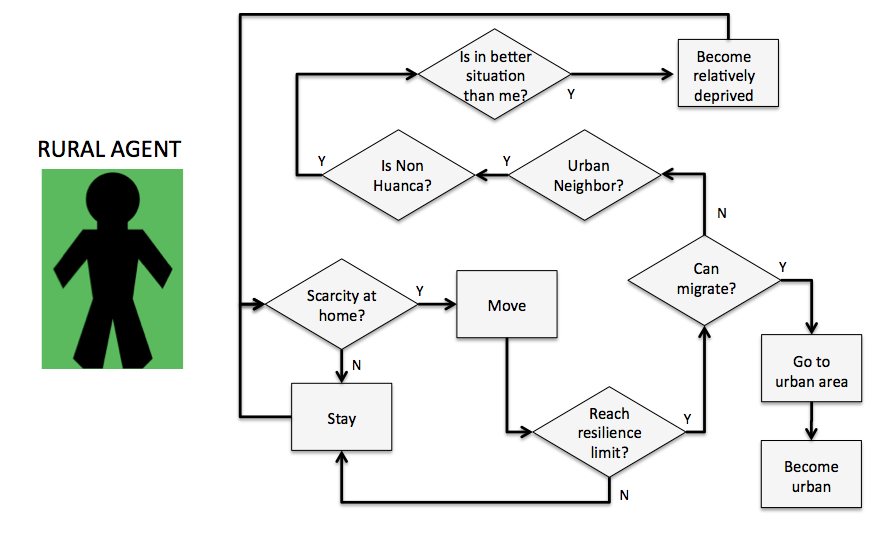
\includegraphics[width=0.8\textwidth]{ruralLogic}
  \caption[Decision making - rural agents]{Decision making - rural agents}
  \label{ruralLogic}
\end{figure}

Figure \ref{urbanLogic} is a flowchart representing the decision making of an urban agent. Similar to the previous figure, the decision flow starts when the agent detects scarcity following a Bayesian approach. Once the agent detects scarcity, he will look for a place to move. As long as the agent detects scarcity where the agent is staying, the agent will move. The moving will end when the agent reaches the resilience limit. If the urban agent can migrate, the urban agent will migrate to the coast or the jungle, depending on the agent's characteristics (employed, educated, marital status). Agents that could not migrate are candidates to feel frustrated. Once the agent is frustrated, the agent will try to connect to other agents in the same situation. These connections make a social network of frustrated or angry agents. A link is destroyed when a member of the network of frustrated agents migrates.

\begin{figure}[ht]
%%\figSpace
\centering
  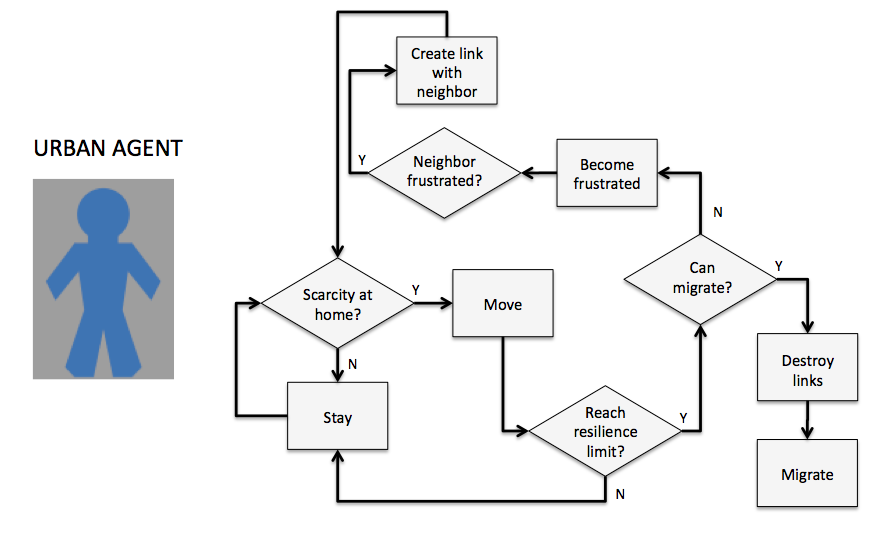
\includegraphics[width=0.7\textwidth]{urbanLogic}
  \caption[Decision making - urban agents]{Decision making - urban agents}
  \label{urbanLogic}
  %%\figSpace
\end{figure}

\clearpage
\subsection{Analysis of Results}


% \begin{quote}
% \emph{``Although policymakers cannot draw lessons from events that have yet to occur, they can try to anticipate events. In doing so, they may treat the future as an extension of the present in order to bound speculation by existing knowledge. Theorists can claim future success for their prescriptions on the grounds that predictions follow logically from premises, whether or not their premises are plausible. Politicians can exploit uncertainty about the future by willfully asserting faith in their proposals, which have yet to be proven wrong (pp.91)''\parencite{rose_lesson-drawing_1993}}
% \end{quote}

% This quote from Professor Richard Rose\footnote{Director of the Center for the Study of Public Policy at the University of Strathclyde, Glasgow} has inspired greatly the purpose of this research. In his work ``\emph{Lesson-Drawing in Public Policy: A Guide to Learning Across Time and Space}'' 
Rose \parencite{rose_lesson-drawing_1993} believes anticipation allows policymakers to forgo the necessary rigors of empirical evidence, as anticipation is not a scientific endeavor but in fact a \emph{political tool} that can be used when facing uncertainty and novelty. This ABM results may halp anticipate a critical situation:

\begin{itemize}
\item {\bf Take one}. The model has been verified and validated. All the population is situated in the \emph{year zero} and the model is ready to run (after last census in 2017). The population count reflects a proportion of actual population. The areas are also proportional. The Glacier Huaytapallana area in in the year zero is represented by the zone in white, the rural settlers inhabit the green area and the urban agents are in the gray area. The water balance is not an issue yet, the water supply is enough for the population water needs. See Figure \ref{esc} (a).

% \begin{figure}[h]
%   %\figSpace % This adds separation
%   \centering
%   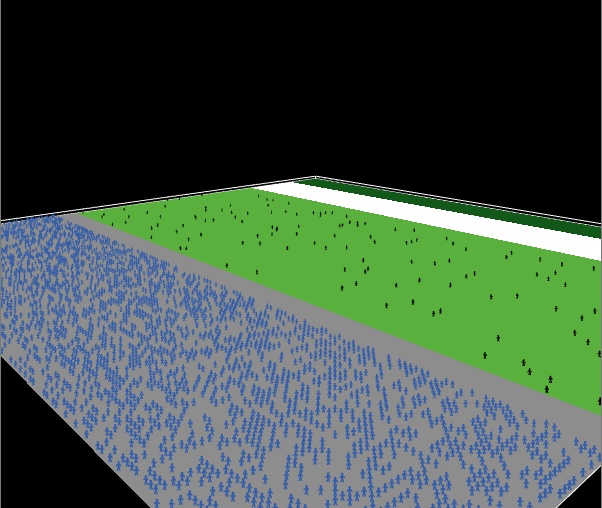
\includegraphics[width=0.5\textwidth]{esc1}
%   \caption{Start of the simulation}
%   \label{esc1}
%   %%\figSpace % This adds separation
% \end{figure}

\item {\bf Take two}. As time passes by, the glacier keeps melting following the identified trend. The pink patches near the white patches represent the zone retreated. Even though there are no water issues in this moment, people started slowly moving away from the more densely populated area (left gray area) into the periurban area. The main driving force for this is the population growth. See Figure \ref{esc} (b).

% \begin{figure}[h]
%   %\figSpace % This adds separation
%   \centering
%   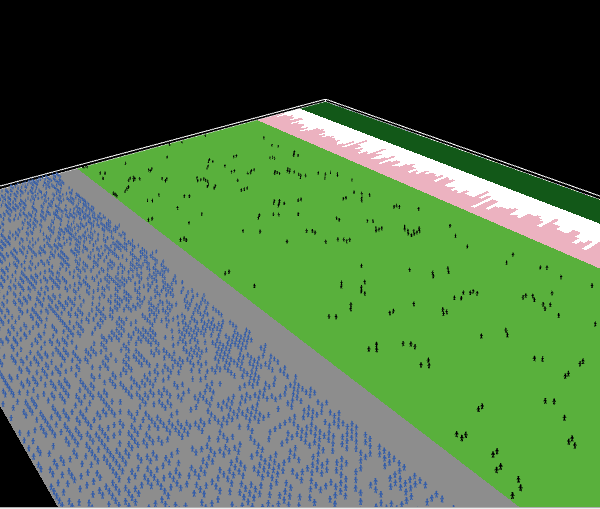
\includegraphics[width=0.5\textwidth]{esc2}
%   \caption{Melting of the Huaytapallana}
%   \label{esc2}
% %  %\figSpace % This adds separation
% \end{figure}

\item {\bf Take three}. The glacier has retreated almost completely, and the water balance for the urban area is now negative. The pink patches in the urban area are affected by the drought during the \emph{dry season}. The drought is felt progressively from the highest risk zones (leftmost gray zone).  If an agent is living in a patch that suffers drought, he may need to move away, depending on his beliefs of future scarcity. There are some urban agents that could not migrate when their resilience was reached. They are already organizing into a network. The peri urbanization process continues but no rural is feeling relatively deprived yet. See Figure \ref{esc} (c).

% \begin{figure}[h]
%   %\figSpace % This adds separation
%   \centering
%   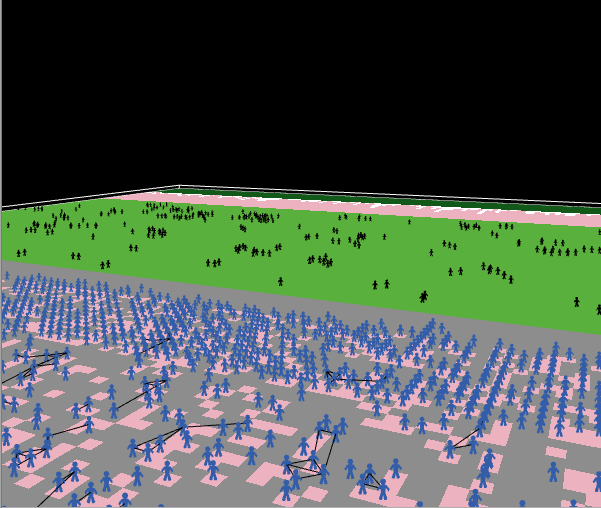
\includegraphics[width=0.5\textwidth]{esc3}
%   \caption{Water scarcity and network of urban people frustrated}
%   \label{esc3}
% %  %\figSpace % This adds separation
% \end{figure}

\item {\bf Take four}. The Huaytapallana has melted completely. This has made the situation even worse during the dry season. Urbans are populating more the periurban area, and the increasing presence of immigrants has started making rurals  feel relatively deprived. The rural agents with a bigger size represent those rural agents. Even though the migration into the coast or the jungle has been massive, there are still many people feeling frustrated living in the area. Not every frustrated urbanite is connected to one another, but there are many network components and cliques every where in the city. The simulation is about to finish after representing 50 years. The potential for conflict and migration turn into a fact in the model. See Figure \ref{esc} (d).

% \begin{figure}[h]
%   %\figSpace % This adds separation
%   \centering
%   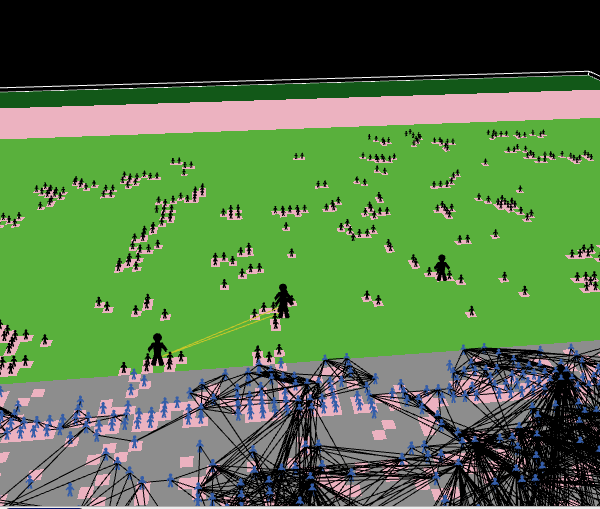
\includegraphics[width=0.5\textwidth]{esc4}
%   \caption{Water scarcity, urban people frustrated and relatively deprived rural settlers}
%   \label{esc4}
% %  %\figSpace % This adds separation
% \end{figure}


\end {itemize}


\begin{figure}[h]
    \centering
    \subfigure[]{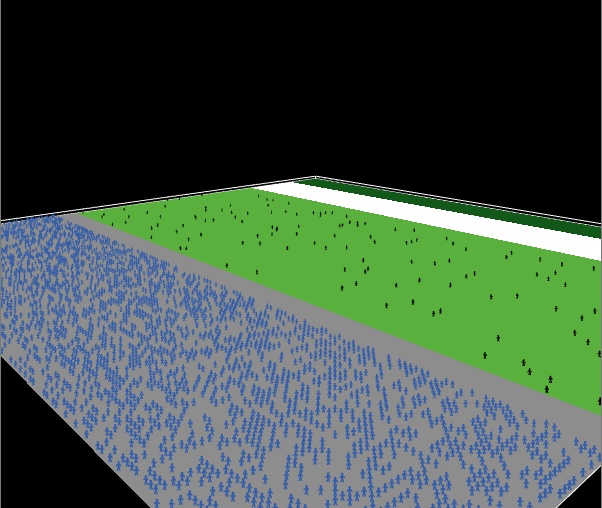
\includegraphics[width=0.4\textwidth]{esc1.png}} 
    \subfigure[]{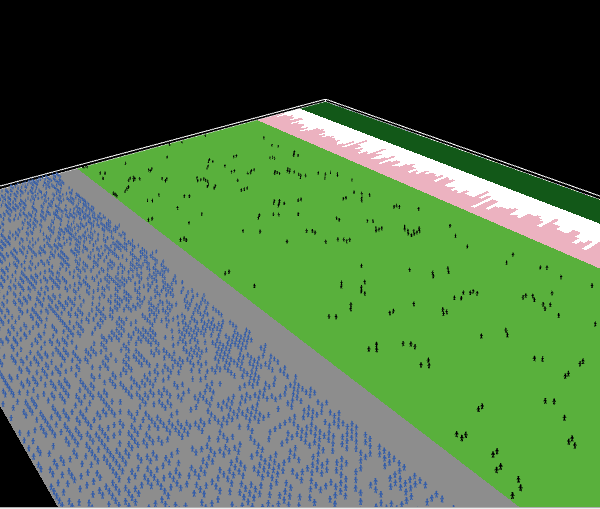
\includegraphics[width=0.4\textwidth]{esc2.png}} 
    \subfigure[]{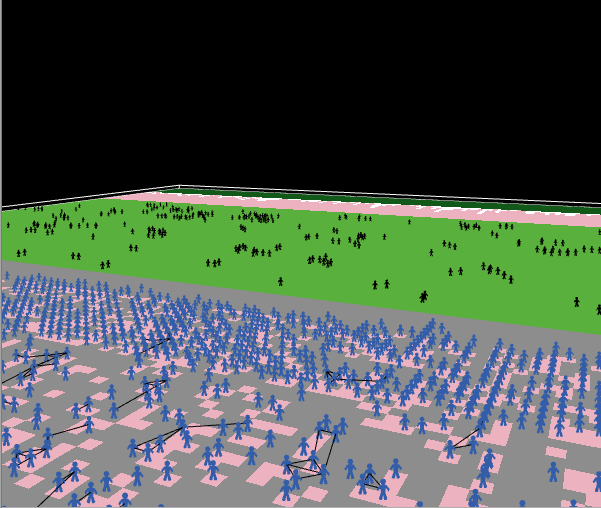
\includegraphics[width=0.4\textwidth]{esc3.png}}
    \subfigure[]{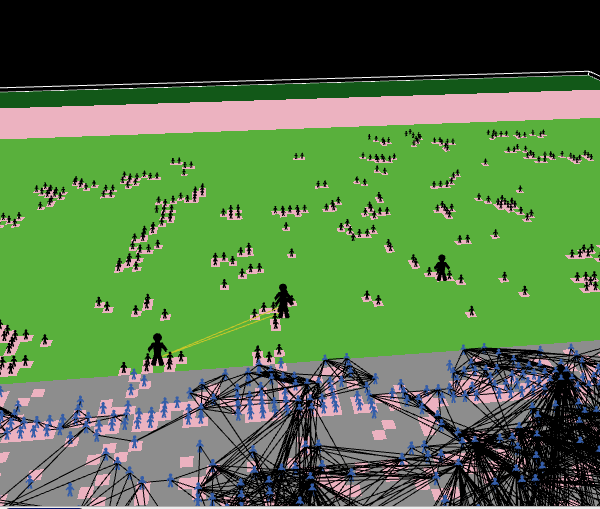
\includegraphics[width=0.4\textwidth]{esc4.png}}
    \caption{(a) Take one (b) Take two (c) Take three  (d) Take four}
    \label{esc}
\end{figure}

Let's try some answers to our initial questions.
% \clearpage

\section {Is drastic migration possible?}

Related to migration, Table \ref{migra-out} informs the final values obtained. There, one can see that, even though it is possible for rurals to migrate, the balance of water in the urban area the next years would not be an issue, so even though migration is allowed for rurals in the code, no immigration took place. Migration started at period 54 (year 27) and the most dramatic migration happened in moment 64, 10 periods later (year 32). If the demographic conditions held true, the migration to the jungle would be the most alarming.

\begin{table}[ht]
\renewcommand{\arraystretch}{1.5}
  %\tableSpace % This adds separation
%  \centering
  \caption{Migration-related results}
{\scriptsize
% latex table generated in R 3.0.2 by xtable 1.7-3 package
% Fri Jul 17 19:25:22 2015
\begin{tabular}{m{5in}p{0.5in}}
  \hline
Variable & Value  \\
  \hline
People that moved to the Jungle & 2662 \\
  People that moved to Lima & 356 \\
  Rural people that moved to urban area &   0 \\
  Moment Migration started &  54 \\
  Max amount that emigrated in a year to the Jungle & 337 \\
  Max amount that emigrated in a year to Lima &  54 \\
  Max amount that emigrated in a year & 391 \\
  Moment when Max amount that emigrated in a year was reached &  64 \\
  Moment when Max amount that emigrated in a year to the Jungle was reached &  64  \\
  Moment when Max amount that emigrated in a year to Lima was reached &  64 \\
   \hline
\end{tabular}}
\label{migra-out}
 % %\tableSpace % This adds separation
\end{table}


\section {Is social conflict possible?}


The Table \ref{conflict-out} informs that the simulation ended with a immigrant  population representing 72\% of the total population, that is, after 100 periods (50 years), the immigrant population share doubled. It is also clear the share of rural people has reached 16\% (an increase of 12\%). An important value to consider is that only 3 people felt relatively-deprived, however that may include their families in case of conflict.

\begin{table}[ht]
\renewcommand{\arraystretch}{1.5}
  %\tableSpace % This adds separation
%  \centering
  \caption{Conflict-related results}

% latex table generated in R 3.0.2 by xtable 1.7-3 package
% Fri Jul 17 19:25:27 2015
{\scriptsize
\begin{tabular}{m{5in}p{0.5in}}
  \hline
Variable & Value \\
  \hline
Max amount of angry people reached & 2497.00\\
  Density of Angry Network when max amount of angry people reached & 0.01\\
  Average clustering coefficient of Angry Network when max amount of angry people reached & 0.41 \\
  Number of network components when Max amount of angry people reached & 491.00 \\
  Moment when Max amount of angry people reached & 96.00 \\
  Rural population when max amount of angry people reached & 569.00 \\
  Urban population when max amount of angry people reached & 3116.00 \\
  Moment that first rural started feeling relatively deprived & 80.00 \\
   \hline
\end{tabular}
}
\label{conflict-out}
  %\tableSpace % This adds separation
\end{table}



Table \ref{conflict-out} also informs that the possibility of conflict in the rural area started around the period 80 (year 40). On the other hand, in the urban area the network of angry people does not get to reach high values, which means that even though there are many angry people, very few of them are connected. However, that result should need further reflection. These results could get the reader wrong if no other measure of connectivity had been obtained. Fortunately, we are aware that the low density does not mean a low potential for conflict, but that there are many components, some of them very tightly connected that could make and escalate conflict. A sample network in a moment of maximum angry people is shown in Figure \ref{network}, showing how unmanageable this situation could become.

\begin{figure}[h]

  \centering
  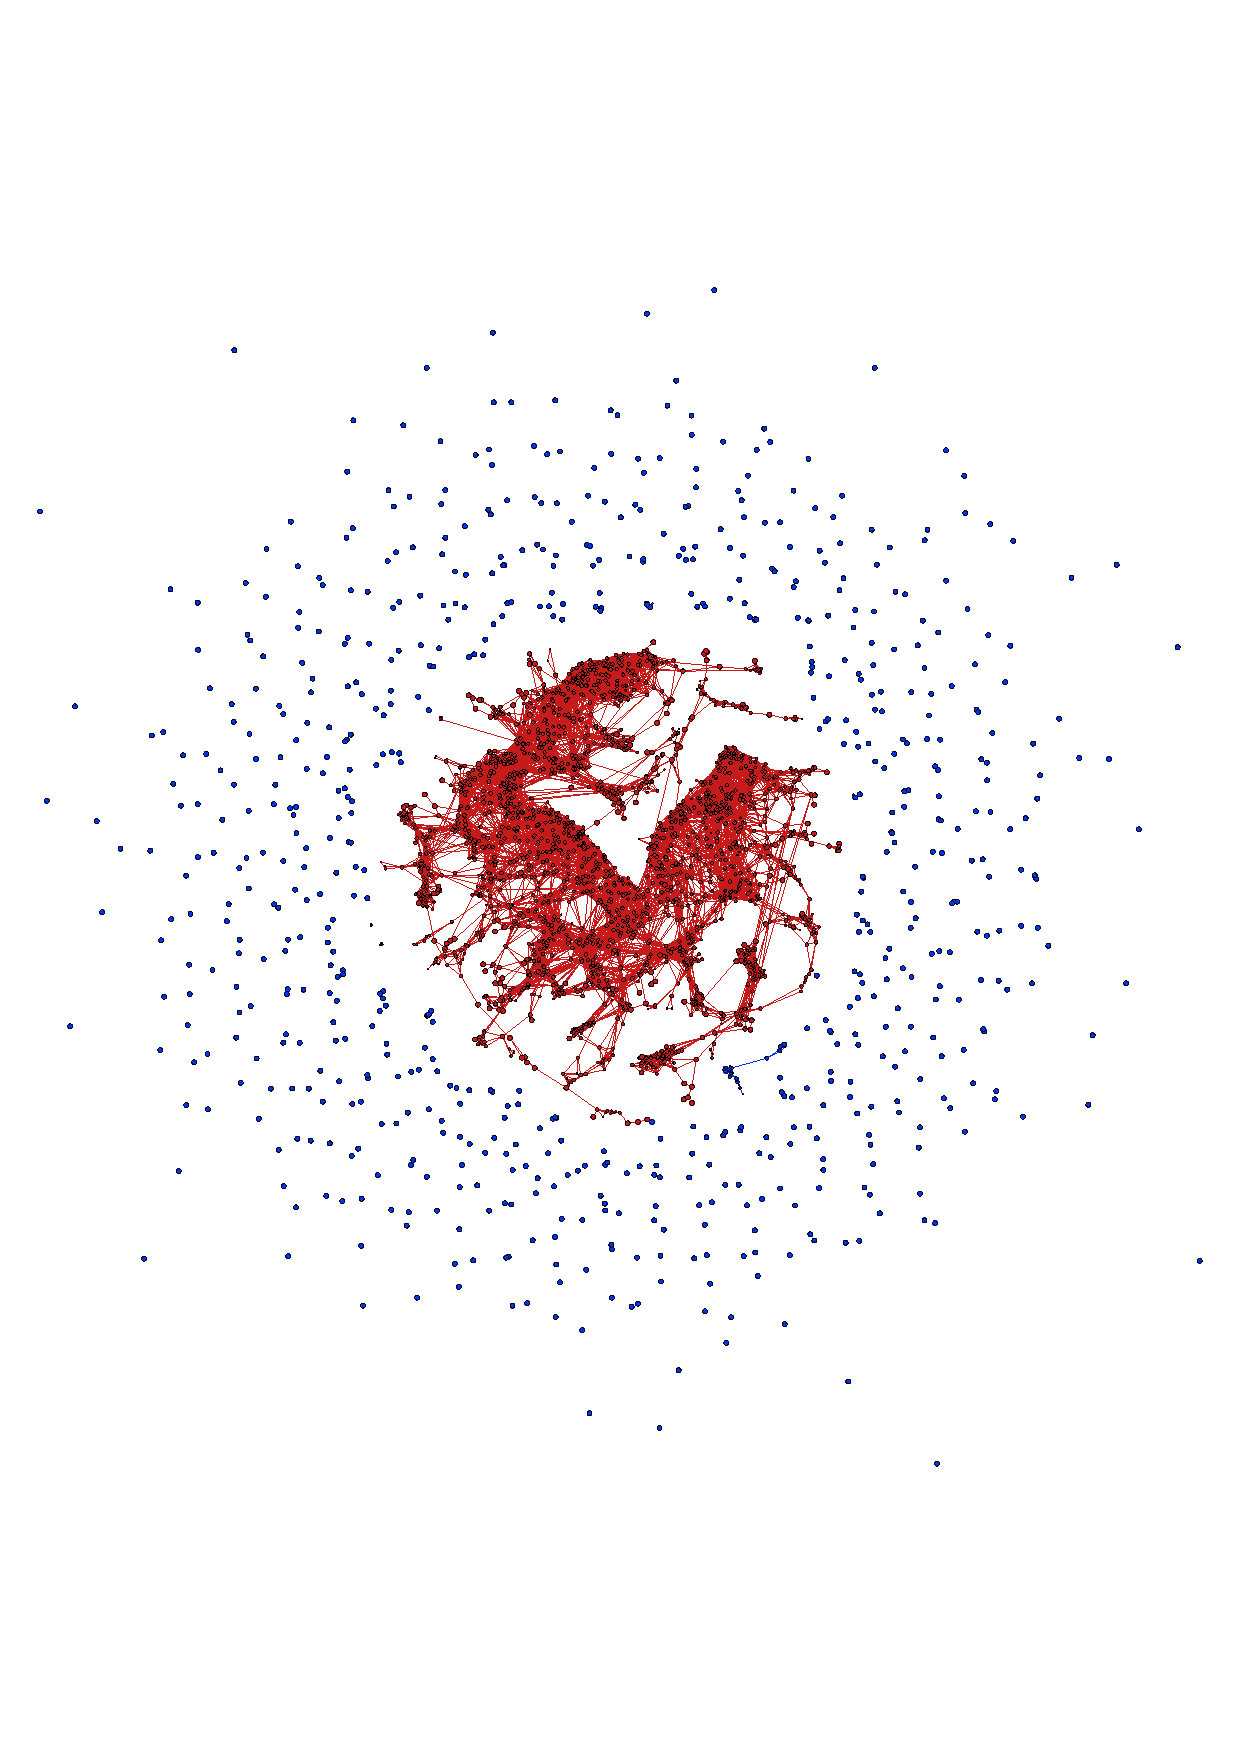
\includegraphics[trim = 0cm 5cm 0cm 5cm,clip,width=0.75\textwidth]{network}
  \caption[Network of Angry People]{Network of Angry People. This is a network during the moment when the maximum amount of angry people was reached. You can see isolates and  components. This network has an average clustering coefficient= 0.3635, 705 connected components and a density = 0.007}
  \label{network}
  %\figSpace % This adds separation
\end{figure}



\section{Discussion and Conclusions}

The natural barrier to anticipation is a reactive mindset, which is very common in policy making \parencite{torjman_what_2005}. For sure, one can not blame decision makers for being reactive as generally the political institutions are a set of rules that have been conceived based on what is known. There may be many examples of catastrophes that could have been avoided if the right anticipatory measure had been taken previously, but it is also true that the legal systems generally lack means to make decision makers liable for their lack of planing; and  only electoral means are a way to express the general discontent for their lack of proactiveness. However, electing a new or better political leader does not undo the damage and suffering of the affected people. A reactive system of policies is not completely bad, and could even be considered an efficient way of spending public moneys. However, when combined with other factors, the whole situation can become catastrophic.

A first negative ingredient can be extremely centralized systems or weakly decentralized. A centralized system will react only after every institution beneath has considered that there is a need for anticipation, and a weekly centralized system gives the local institutions the illusion of decision making, when in reality there is a regulation that will force the local authority to deal with a complicated set of institutions. The Shullcas and the Huaytapallana may be clearly affected by this situation. Another negative ingredient to reactive policy-making is symbolic and superficial proactiveness. Particularly when dealing with this climate change issue, programs and organizations are created, technical documents are produced, presentations and dinners are offered, but at the end of the day there are no real measures beyond declarations of concern.

The level of economic development is also a key factor in understanding the ability to cope with water shortages, as more developed countries have more technological and financial resources to deal with drastic environment issues. Poorer regions, countries, or localities have meager funds and often suffer through political instability that constrains implementation of effective and long-lasting policies. However, economic development has not stopped advance economies like the USA to be reactive in many cases in many different issues like the Challenger accident, the 9/11, Katrina hurricane, and so on (for more stories see \parencite{bazerman_predictable_2004}). Then, poor leadership affects enormously a reactive system of policies. A poor leader plays safe, and tends to leave difficult situations to \emph{experts}, framing complex issues as \emph{technical}. As explained by Heifetz and Linsky \parencite{heifetz_leadership_2002},
once leaders frame a complex problem as technical instead of complex-adaptive the political system just does ``routine management'' instead of ``change management''. This explains that the reports on the watershed appeared around 2010, and all of them were very technical; and since then, no more knowledge on this area has been produced from the government.



\section{Beyond the model}

{\bf What should be improved in the model?} \\
Every model needs assumptions and facts, those facts can be qualitative or quantitative, and this agent-based model has dealt very well with facts and assumptions. However, the most urgent areas of improvement can be:
\begin{itemize}
\item Have a better sub model of what an agent could do when it predicts water scarcity is important. In our model, the agent looks for another sources of water, and when the agent finds a better place it abandons its home and moves to another place within the system, and keep doing that until his desire to stay in the system is surpassed. However, we would have preferred to have information on neighborhoods and its economic capacity, to implement an algorithm considering that information, but that data does not exist. An important investment would be needed to produce that data.
\item This model assumes thta the coas or jungle are the main destinations for the emigrants, but coast in fact represents ``big cities in the coast'' and the jungle represents ``good places to go if you are a risk taker and your are not planing to bring your family''; although the answers from the interviews mentioned these two places it would be important to expand the model and see how the new arrivals are received and what new issues arise in those destinations. The answers also mentioned ``foreign countries'', but that destination has not been included (but ``coast'' could represent it).
\item It would be important to consider more strategies of the agent according to its economic capacity. The economic capacity is unknown at agent level, so further work on this should be done. It is important also to conduct a more detailed analysis on water regulation from the government to get the agents reduce consumption; since Peru is a country where no political authority wants to alter the price of water (water is very cheap in Peru), a different regulation mechanism should be thought following a participatory approach.

\item A different programming platform could be important to consider. At this point, we have reached the capacity of the program NetLogo\parencite{wilensky_introduction_2015} but if this model becomes more computing-intensive, there is a clear need to migrate the model into more sophisticated platforms such as Mason \parencite{luke_mason_2015}, Repast \parencite{north_complex_2013}, or Gamma \parencite{taillandier_building_2019}. In fact, the code is ready to be sent to real maps, and see the simulation in a more realistic setting, but those other ABM platforms are needed to make the conversion useful.
\end{itemize}




{\bf What measures should be taken?}

This model, despite the real data that has been used to feed it, is still more a political tool than a engineering one. Its purpose is to show potential and not clear forecast of counts and moments, but a clear picture of what might happen and what to do to avoid it or gain time. This model's ultimate goal is to raise enough awareness that triggers real political action. With that in mind, there are some recommendation on the next steps policy makers should follow:

\begin{itemize}
\item \emph{Make sure people in rural area have enough rights and mechanisms to stay in their lands in good conditions.} The tendency of immigration may not diminish in the short run and rural people have no intention to leave Huancayo. To avoid relative deprivation emerge, policy makers from the central government need to assist rural populations to adapt their farming practices; regional planers need to determine buffers that separate urban from rural area as well as assure minimal literacy conditions; while local governments need to stop giving building permits in the buffer area. The local University may also contribute to raise competitiveness of the local production.

\item \emph{Create mechanisms to ensure political participation of rural people.} Rural people are politically under represented. They only have local committees that regulate their internal activities in the community; but they have no real presence in the regional decision making. Local and regional governments should make sure that rural people have voice in every meeting held monthly where their participation will avoid future discrepancies. Policy makers have to keep in mind that the model is constantly recommending to increase the water reserve from the rainy season, which will need investment and the use of arable and/or herding land; in either case, rural communities will feel they are affected to favor exclusively the urban.

\item \emph{Improve participatory water governance.} The distribution of water between rural and urban area is currently a process that represents a constant debate. From the interviews, rural people believe that the city is taking more than water than they should from the Shullcas during the dry season and that the rural needs are relegated due to the pressure of the urban majority. Water management has many actors involved, including two Ministries from the central government (Agriculture and Environment), but the technical criteria adopted so far is biased toward the needs of the urban area.


\item \emph{Create and save the institutional memory.}This model has been done in the USA, but very distant from the modeling conditions we are familiar. Developed countries have long understand the importance of collecting, organizing and sharing data for the research community to find research problems and propose different solutions, or more importantly, to keep a memory of the events a community has experienced and help their local analysts do their job. Peru is the opposite.

\item \emph{Do not hide the crisis, but show a plan.} The dramatic situation has to be shared with the population, but in a message that shows the local governments have a plan that needs urban people to alter their inefficient use of water, or to learn routines that avoid unnecessary use of water. If the water demand decreases in the long run, make sure this process gets as slow as possible. For that, different campaigns should be promoted at elementary and high school level to be more efficient using water in the future generations of \emph{Huancainos}; organize contests at college level to promote local inventions; and organize neighborhood contests to demonstrate how to achieve efficient practices in the use of water.

\item \emph{Seek collaboration from civil society, especially research institutions.} The highlands of Peru have been always scenarios for NGOs to operate. Ideally, NGOs detect social problems and work with the community to empower their actors; but this time the challenge is different, as it deals with the resilience and adaptive capacity of people facing high uncertainty of the future environmental conditions and the reactions their neighbors themselves will have in those critical moments. In this situation, the production of more knowledge is needed as well as interdisciplinary debate. The government has serious limitations to hire people permanently, but the local public University is the forgotten partner that could make all the difference. The local University has enough resources to fund important programs that can keep updating the social and natural situation for more informed policy making and modeling, and which should create mechanisms for a two-way knowledge transfer, that is share scientific knowledge and collect traditional knowledge.
\item \emph{Be careful of easy solutions.} This work has suggested many times the saving of water. This is a decision that needs to be very well planned. To start, a huge reservoir for the area seems to be a good solution, but decision makers have to be aware of the Huaytapallana failure. This failure can cause any time a huge earthquake, and a huge reservoir represents a great potential for disaster. The saving of water will need a lot of work from the political class and the people themselves. From the top down, the infrastructure to save or become more efficient should be built; and the urban and rural settlers have the responsibility to be more efficient using water. Another important way to secure water will be a better management of the ground water, which currently is used without detailed knowledge of its quantity nor quality, and without any recharging policy.

\end{itemize}

. %For multi-author works \parencite[e.g.,]{Multiauthor2020}, the full author list will be included the first time. However, on subsequent reappearances of that reference, it will be shortened as APA intended \parencite{Multiauthor2020}.
% For whatever reason, it does not seem like the multi-author work \parencite[e.g.,][]{Multiauthor2020} is working as it should, where it gives the full list the first time it is included in text, then truncates afterwards \parencite{Multiauthor2020}. I am not sure what is up with that, so the best advice I can offer you is to do write out the first instance yourself, then let \LaTeX{} handle the rest. It sucks, I know. Such is the nature of the \LaTeX{} beast, sometimes.
% 
% As a formatting note, the References page needs to start on a new page. This \textit{should be} handled automatically by \LaTeX{}, but it's still useful to know the format.
% 
% While I have your attention before diving into the sections, something that may slip by unnoticed is the \LaTeX{} quirk about quotation marks. If you were to include a quote using the regular quotation marks, "it will look like this." However, the \LaTeX{} specific way of doing it, that just gives it that little bit extra flair, is to use a double tick mark (on the tilde key up on the number row) to start the quote, and a double apostrophe to close it. That will make the quote ``look like this instead.'' They are ``fun little guys'' hugging your quote, instead of the "more bland marks" you get from the regular quotation marks.
% 
% To close out this section, I will finally talk about the contents of the Introduction. In these sorts of papers, think of the information process in the shape of an hourglass (stay with me, it'll make sense). The general idea is that you start at the broadest point, work your way into more and more specific, until you are at the point of this paper - the theory its testing and the hypothesis. Then you stay in that specific level of detail through the Methods and Results. The Discussion starts specific (i.e., what you did or did not find), then work your way back out to the broader meaning or implications. 
% 
% \section{Method}
% 
% \subsection{DELETE THIS SECTION - this is an informative section, not something to be included in your final paper.}
% 
% I have tried to include the most I've seen asked of students in these papers. You may not need to fill out all of these boxes, in which case you can just delete them. Along with this subsection.
% 
% Also, I have seen many different combinations of these boxes - e.g., in one of my papers, I had a ``participants and materials'' section followed by a ``procedure and measures,'' but cannot remember why it was written that way. Maybe it is what the journal wanted? Moral of the story here: go with what the person who is making the decision about the quality of your paper wants. If they want everything in its own little box, do it. If they want some boxes combined, do that.
% 
% Just make sure you delete or comment out this subsection!
% 
% \subsection{Participants}
% 
% Talk about the people who participated in your study. How many students, sourced from where, reimbursed how, ethics assured by what?
% 
% \subsection{Materials}
% 
% What materials were used in the course of this experiment? Try to walk the line between being overly specific (i.e., ``pens were standard Bic Clio Stic of medium thickness'') while still having enough detail someone else could read your paper and replicate what you used.
% 
% Sometimes it can be helpful to include the stimuli used in the experiment. For example, here is an example table (Table \ref{tab:table_words}) of words that were used in this hypothetical experiment. If you make use of the label command, \LaTeX{} will handle numbering things for you.
% 
% % There's lots of little components to the table. For the most part you can just copy it, or build your own with Overleaf's table wizard up top.
% % I'll mention that the & character separates items into different columns on a row, and the \\ ends that line. \hline generates a line that matches the width of the table.
% \begin{table}
%     \caption{Sample words from this hypothetical experiment.}
%     \centering
%     \begin{tabular}{cc} %The c's here indicate the columns will be centered
%         \hline
%          First word & Second word \\
%          \hline
%          Yeet & Yoink \\
%          Hot & Lit \\
%          \hline
%     \end{tabular}
%     \label{tab:table_words}
% \end{table}
% 


% 
% \subsection{Measures}
% 
% This sets up what measure(s) you took during your experiment, including information about \textit{how} those measures were gathered. Was it with some form of worksheet? Was it collected electronically? If electronic, was it through a website or something like E-Prime? If a keyboard was used, were there any specifics about the keys used?
% 
% \subsection{Design}
% 
% This is typically used to describe the conditions of the experiment. Did everyone experience the same things throughout the experiment, or were there counterbalances, such as for item order exposure, condition order exposure, conditions on days, etc.? 
% 
% For undergrad research projects, lab instructors generally try to encourage students towards easier projects, as analyzing a 3 x 2 x 5 experiment is rough, no matter how far along the academic process you are. So I would expect to see something more along the lines of a 2 (experimental manipulation) x 2 (order counterbalance) design.
% 
% 
% \subsection{Procedure}
% 
% From the time the participant starts the experiment to the time they leave, what did they experience? After informed consent was obtained, what did they do? Or, in some cases, what did you do to them? \textit{What did you do to them?} Make sure you highlight parts where things may deviate from the norm, such as in the debrief, needing to reveal to participants they hadn't been informed of the full nature of the experiment earlier as it would have impacted their ability to respond honestly or otherwise contaminated the data.
% 
% 
% 
% \section{Results}
% 
% Some instructors will want things broken down with the subheadings (e.g., `Descriptive Statistics') I have included, some will light your paper on fire if you \textit{do} include these. Always check with the assignment/rubric for what is wanted. Also, don't check my math on these, I am making all of the numbers up as we go, so it's almost certainly not going to hang together correctly.
% 
% I'll add this tip in here: since \LaTeX{} uses the percent symbol as the signal to comment out/hide what's typed after it in that line, what do you do if you need that symbol? You add what's called the `escape character' in front of it - the backslash. So, it would look like this: 21\%. Boom, you've got a percent symbol in text. Same goes for an ampersand: \&.
% 
% \subsection{Descriptive Statistics}
% 
% In this portion, you describe the data obtained. This includes things like the counts, means, and standard deviations. This may be omitted or rolled into the rest of the statistical discussion, so as always, check with what is being asked of you. If it is wanted as a separate section, check to see if it would be acceptable to include things as a table, a figure, or if it would be better to write it out in text. We are going to use a figure.
% 
% \begin{figure}
%     \centering
%     \includegraphics[width=0.75\linewidth]{sampleFig.png} % This is setting the figure to be .75x the width of the line. This can go all the way from 0.1 to 1 (and beyond, but then you're outside the page).
%     \caption{The mean vibes for each word type and counterbalanced condition order. Error bars represent one standard error of the mean.}
%     \label{fig:OverallEffect}
% \end{figure}
% 
% Figure~\ref{fig:OverallEffect} shows the means and standard errors for the four experimental groups. As shown, the mean vibes for the second word ($M = $ 69, $SE = $ 7.5) were greater than the first word ($M = $ 42, $SE = $ 3), but roughly equivalent between presentation order conditions. Another fun little \LaTeX{} thing here: your instructor may explicitly want you to use $M$, but one of \LaTeX{}'s strengths is the easy of ``math mode'' (i.e., everything enclosed by the dollar signs). %In math mode, you can easily throw in Greek characters. So you \textit{could} instead present the descriptive statistics as ($\mu = $ 42). Oooh. Shiny. Although that seems to make Overleaf work extra hard, so I keep seeing a message encouraging upgrading to a paid plan, so I've commented this part out.
% 
% \subsection{Inferential Statistics}
% 
% This is where you start to do the actual statistical analysis. We generally tell students not to \textit{interpret} what the results mean until the discussion, but pay attention when reading journal articles - realistically a bit of interpretation does tend to happen at this point in published works.
% 
% A benefit of using \LaTeX{} is the ease in adding in macros to simplify your life. A common place I rolled these out in my dissertation were to make the formatting of all the analyses correct without a lot of work. I will include a couple example macros in the editor-side now, then use them in text. But, \textbf{another pro tip:} if you are going to deploy these macros, I would get in the habit of putting them up in the preamble so they are easier to find. Also, if you really get on board the \LaTeX{} train (which you should), you can recycle the preamble between projects, so those macros will also come along for the ride.
% 
% % A macro will have this format \newcommand{macroNameYoullUseToCallIt}[Number of inputs]{What the macro does} 
% % The #s indicate where information will be slotted in when the macro is used
% % The dollar signs indicate "math mode" is being used. It's mandatory for some functionality (like super/subscripts) or accessing the Greek alphabet used in statistical reporting.
% % These macros are including the amount of info we expected from students when I was TAing labs. You can fill them out further if more info is required - just make sure you update the number in the square brackets!
% \newcommand{\ttestSig}[2]{$t$(#1) = #2, $p < .05$}
% \newcommand{\ttestInsig}[2]{$t$(#1) = #2, $p > .05$}
% \newcommand{\anovaSig}[3]{$F$(#1,#2) = #3, $p < .05$}
% \newcommand{\anovaInsig}[3]{$F$(#1,#2) = #3, $p > .05$}
% 
% Using the hypothetical experiment we have set up, let's say there was a significant interaction found between the word conditions (first versus second) and exposure order (first-second versus second-first), \anovaSig{11}{111}{4.20}. Pairwise comparisons indicate that this was driven by the words themselves, as there was a significant difference between the words, \ttestSig{111}{3.21}, but not for the exposure order, \ttestInsig{111}{.42}.
% 
% \section{Discussion}
% 
% As mentioned at the close of the Introduction, the Discussion starts out specific before building out to the broader picture. This will typically mean that the discussion starts with a reiteration of the Results, with more emphasis on interpretation. What differences were (or were not) found? Does this support your predictions, or have you failed to reject the null hypothesis? Statements of that nature.
% 
% With that done, you can work to tie your findings into the existing literature. Perhaps this result supports the work of \textcite{Contributor2023} but contradicts others \parencite[e.g.,][]{Sample2024}. %The extra square brackets here are telling LaTeX that the e.g., needs to be in front; it seems to assume otherwise that the e.g., belongs after the citation. Also note that I can have this comment here without breaking the paragraph. You need a double line break to separate paragraphs.
% Why might this be the case? What similarities or differences exist between your experiment and the other works that could explain the differences? Or if the results are similar, what does this mean for the core theory (e.g., demonstrates it held up with different stimuli, or in a different context, or with different timing, etc.).
% 
% It is also important to work in potential limitations of your work. Frequently in undergrad cognitive lab reports, this will involve the sample size. It can be hard to reach significance when you have a sample size of 10. Other common limitations can be things like the stimuli didn't work out as you had hoped, the participants didn't understand the experiment directions (or were savvy to what you were testing which biased their data), or things you notice in running the experiment that you would do differently if you redid it in the future.
% 
% Finally, close things out by reiterating the brief version of your findings, what it means for the theory you were testing, and what it could mean for future research. Happy writing!
% 


\printbibliography

\end{document}

%% 
%% Copyright (C) 2019 by Daniel A. Weiss <daniel.weiss.led at gmail.com>
%% 
%% This work may be distributed and/or modified under the
%% conditions of the LaTeX Project Public License (LPPL), either
%% version 1.3c of this license or (at your option) any later
%% version.  The latest version of this license is in the file:
%% 
%% http://www.latex-project.org/lppl.txt
%% 
%% Users may freely modify these files without permission, as long as the
%% copyright line and this statement are maintained intact.
%% 
%% This work is not endorsed by, affiliated with, or probably even known
%% by, the American Psychological Association.
%% 
%% This work is "maintained" (as per LPPL maintenance status) by
%% Daniel A. Weiss.
%% 
%% This work consists of the file  apa7.dtx
%% and the derived files           apa7.ins,
%%                                 apa7.cls,
%%                                 apa7.pdf,
%%                                 README,
%%                                 APA7american.txt,
%%                                 APA7british.txt,
%%                                 APA7dutch.txt,
%%                                 APA7english.txt,
%%                                 APA7german.txt,
%%                                 APA7ngerman.txt,
%%                                 APA7greek.txt,
%%                                 APA7czech.txt,
%%                                 APA7turkish.txt,
%%                                 APA7endfloat.cfg,
%%                                 Figure1.pdf,
%%                                 shortsample.tex,
%%                                 longsample.tex, and
%%                                 bibliography.bib.
%% 
%%
%%
%% This is file `./samples/shortsample.tex',
%% generated with the docstrip utility.
%%
%% The original source files were:
%%
%% apa7.dtx  (with options: `shortsample')
%% ----------------------------------------------------------------------
%% 
%% apa7 - A LaTeX class for formatting documents in compliance with the
%% American Psychological Association's Publication Manual, 7th edition
%% 
%% Copyright (C) 2019 by Daniel A. Weiss <daniel.weiss.led at gmail.com>
%% 
%% This work may be distributed and/or modified under the
%% conditions of the LaTeX Project Public License (LPPL), either
%% version 1.3c of this license or (at your option) any later
%% version.  The latest version of this license is in the file:
%% 
%% http://www.latex-project.org/lppl.txt
%% 
%% Users may freely modify these files without permission, as long as the
%% copyright line and this statement are maintained intact.
%% 
%% This work is not endorsed by, affiliated with, or probably even known
%% by, the American Psychological Association.
%% 
%% ----------------------------------------------------------------------
